\section{Resultados}
\subsection{Las redes neuronales como un filtro}
\begin{itemize}
    \item Bode Diagrams
\end{itemize}
\subsection{¿Qué hace la defensa de JPEG?}

Como vimos en la sección de compresión JPEG, cuando esta es aplicada a una imagen que ha sido sometida a un ataque adversario, los componentes de alta frecuencia se eliminan y, así como los humanos percibimos en menor medida dichos componentes, es posible que la red no logre distinguir el ataque perpetrado sobre la imagen, esto debido a que los ataques suelen tratarse de pequeñas cantidades de ruido o distorsión introducidos en la imagen y, al reducir la calidad de la misma, la red tiene más probabilidades de recuperar la clasificación original de la imagen.

En la Figura \ref{jpeg_def} se muestra el resultado de nuestro entrenamiento de las redes LeNet y ResNet utilizando MNIST y el ataque FGSM para distintos niveles de compresión JPEG como defensa. Se observa que, efectivamente, conforme aumenta la compresión (disminuye la calidad), la precisión (accuracy) en la clasificación de las imágenes por parte de la red es mayor.

\begin{itemize}
    \item Intuition: JPEG removes noise that humans can't see
    \item Show graphs of jpeg defense vs epsilon of each attack
    \item Bode diagrams with jpeg conversion as first layer
\end{itemize}

\begin{figure}[h]
    \centering
    \begin{subfigure}[b]{0.49\textwidth}
        \centering
        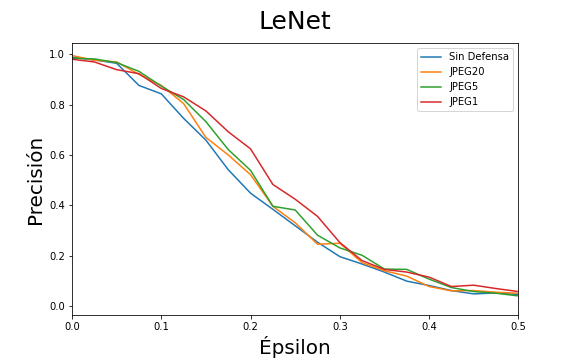
\includegraphics[width=\textwidth]{images/jpeg/jpegdefense_vs_epsilon_linear.png}
        \caption{LeNet}
    \end{subfigure}
    \begin{subfigure}[b]{0.49\textwidth}
        \centering
        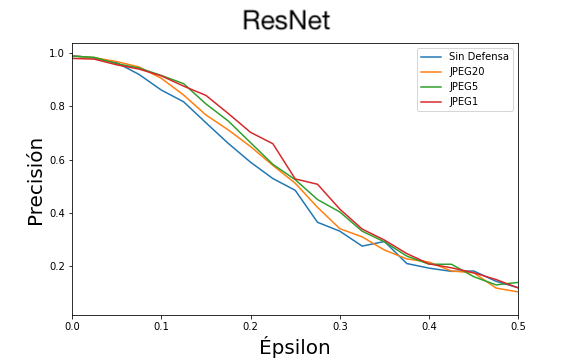
\includegraphics[width=\textwidth]{images/jpeg/jpegdefense_vs_epsilon_nonlinear.png}
        \caption{ResNet}
    \end{subfigure}
    \caption{Resultado de la compresión JPEG como defensa ante el ataque FGSM sobre MNIST}
    \label{jpeg_def}
\end{figure}

\begin{figure}[h]
\centering
\begin{subfigure}[t]{0.22\textwidth}
\centering
    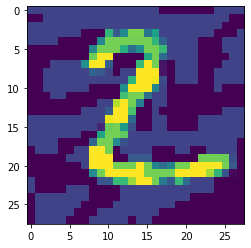
\includegraphics[width=\textwidth]{images/jpeg/fgsm_Le.png}
    \caption{Sin compresión JPEG}
    \label{fgsm_jpeg}
\end{subfigure}
\hspace{1em}
\begin{subfigure}[t]{0.22\textwidth}
\centering
    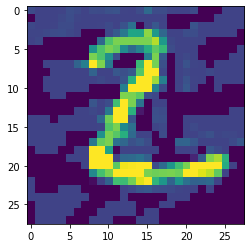
\includegraphics[width=\textwidth]{images/jpeg/fgsm_jpeg20_Le.png}
    \caption{20\%}
    \label{fgsm_jpeg}
\end{subfigure}
\hspace{1em}
\begin{subfigure}[t]{0.22\textwidth}
\centering
    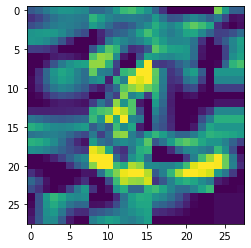
\includegraphics[width=\textwidth]{images/jpeg/fgsm_jpeg5_Le.png}
    \caption{5\%}
    \label{fgsm_jpeg}
\end{subfigure}
\hspace{1em}
\begin{subfigure}[t]{0.22\textwidth}
\centering
    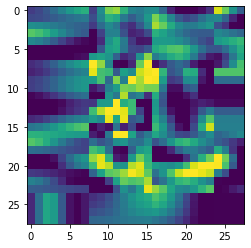
\includegraphics[width=\textwidth]{images/jpeg/fgsm_jpeg1_Le.png}
    \caption{1\%}
    \label{fgsm_jpeg1}
\end{subfigure}
\caption{Ruido del ataque FGSM para distintas calidades en la compresión JPEG}
\label{Noise}
\end{figure}

\subsection{Los Efectos de Overfitting y Overparameterization}
\begin{itemize}
    \item here they suggest overparameterization contributes to sharp gradient landscape \cite{ma2020understanding}...we find the opposite
    \begin{figure}[h]
        \centering
        \begin{subfigure}[b]{0.49\textwidth}
            \centering
            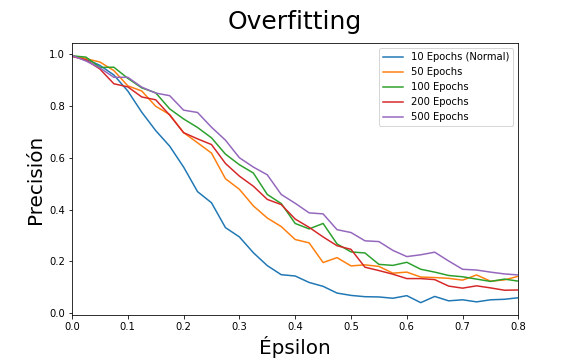
\includegraphics[width=\textwidth]{images/overfit_vs_attack.png}
            \caption{overfitting}
            \label{overfit}
        \end{subfigure}
        \begin{subfigure}[b]{0.49\textwidth}
            \centering
            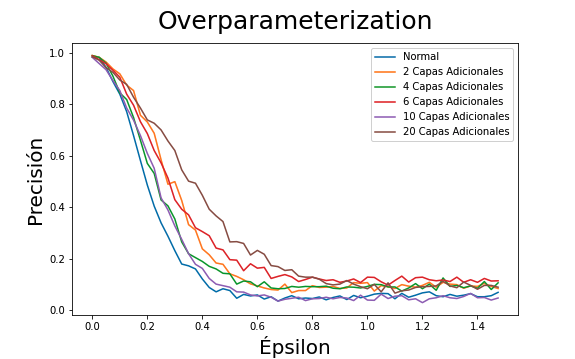
\includegraphics[width=\textwidth]{images/overparam_vs_attack.png}
            \caption{overparameterization}
            \label{overparam}
        \end{subfigure}
        \caption{Efectos}
        \label{overaparam_overfit}
    \end{figure}
    
    En la Figura \ref{overfit} se observa que conforme aumentamos el número de épocas (epochs), la precisión (accuracy) aumenta con respecto a cada épsilon, excepto para 200 épocas, cuya precisión es menor que la de 100 épocas, e incluso menor que la de 50 épocas para épsilon $>$ 0.5. Aumentar el número de épocas implica un sobreajuste (overfitting) de la red neuronal, lo cual significa que...
    
    En la figura \ref{overparam} se observa que conforme aumentamos el número de capas (layers), la precisión aumenta, excepto para 4 y 10 capas adicionales. Nótese que para épsilon $>$ 0.8, la red con 6 capas adicionales tuvo el mejor desempeño. Aumentar el número de capas implica una sobreparametrización (overparameterization) de la red neuronal, lo cual significa que...
    
    \item fix a large overparameterization and see if overfitting has the same effect
    \item pick an overparameterization and overfitting and check jpeg

\end{itemize}
\subsection{Saliency}
\begin{itemize}
    \item show figures from notebook of how adversarial noise attacks parts of the image that seem vulnerable (for example changing a 3$\to$8)
    \item Show Gradient-based localization of both imiage sets and how they change after adding adversarial noise\cite{Selvaraju_2019}
\end{itemize}
